% This LaTeX document needs to be compiled with XeLaTeX.
\documentclass[12pt]{article}
\usepackage[margin=0.8in]{geometry}
\usepackage[utf8]{inputenc}
\usepackage{graphicx}
\usepackage[export]{adjustbox}
\usepackage{amsmath}
\usepackage{amsfonts}
\usepackage{amssymb}
\usepackage[version=4]{mhchem}
\usepackage{stmaryrd}
\usepackage{bbold}
%\usepackage[fallback]{xeCJK}
\usepackage{polyglossia}
\usepackage{fontspec}
\usepackage{censor}
%\setCJKmainfont{Noto Serif CJK TC}
\graphicspath{ {../Images/} }
\usepackage{enumitem}
\usepackage{tikz}
\usepackage{amsthm}
\usepackage{tcolorbox}
\usepackage{array}
\usepackage{tabularray}
\usepackage{makecell}

\tcbuselibrary{theorems}

\definecolor{GrayCen}{HTML}{d2d2d2}
\definecolor{GrayBG}{HTML}{d9d9d9}
\definecolor{BlueDef}{HTML}{104e8b}
\definecolor{GreenProp}{HTML}{025540}
\definecolor{RedMet}{HTML}{cd5556}
\definecolor{BlackSav}{HTML}{000000}
\def\censorcolor{GrayCen}
\let\svcensorrule\censorrule
\renewcommand\censorrule[1]{%
\textcolor{\censorcolor}{\svcensorrule{#1}}}

\newtcbtheorem
  []% init options
  {definition}% name
  {Définition}% title
  {%
    colback=GrayBG,
    colframe=BlueDef,
    fonttitle=\bfseries,
  }% options
  {def}% prefix

\newtcbtheorem
  []% init options
  {proposition}% name
  {Proposition}% title
  {%
    colback=GrayBG,
    colframe=GreenProp,
    fonttitle=\bfseries,
  }% options
  {prop}% prefix

\newtcbtheorem
  []% init options
  {method}% name
  {Méthode}% title
  {%
    theorem name,
    colback=GrayBG,
    colframe=RedMet,
    fonttitle=\bfseries,
  }% options
  {met}% prefix
  
\newtcbtheorem
  []% init options
  {savoir}% name
  {Savoir-faire du chapitre}% title
  {%
    theorem name,
    colback=GrayBG,
    colframe=BlackSav,
    fonttitle=\bfseries,
  }% options
  {sav}% prefix

\newtheoremstyle{break}
  {\topsep}{\topsep}%
  {}{}%
  {\bfseries}{}%
  {\newline}{}%
\theoremstyle{break}
\newtheorem*{example}{Exemple.}
\newtheorem*{remark}{Remarque.}

\newenvironment{demo}[1][\proofname]{%
  \begin{proof}[#1]$ $\newline
}{%
  \end{proof}
}

\setmainlanguage{french}
%\setmainfont{CMU Serif}

\title{
\vspace{4em}
\centering
\tcbset{colframe=BlackSav,colback=GrayBG}
\tcbox[tikznode]{
Chapitre 5 \\Dérivation et applications
}
}

\author{}
\date{}

\setlength\parindent{0pt}
\setlist[itemize]{noitemsep}
\setlist[enumerate]{noitemsep}

\newcolumntype{C}[1]{>{\centering\arraybackslash}m{#1}}
\newcolumntype{L}[1]{>{\raggedright\arraybackslash}m{#1}}
\newcolumntype{N}{@{}m{0pt}@{}}

\begin{document}
\maketitle

\tableofcontents

%\newcommand{\hideM}[1]{\colorbox{gray!50}{\phantom{$\displaystyle #1$}}}
%\newcommand{\hide}[1]{\colorbox{gray!50}{\phantom{#1}}}
\newcommand{\hideM}[1]{#1}
\newcommand{\hide}[1]{#1}

\newpage 

\section{Étude des variations}
\begin{proposition}{(admise)}{}
Soit $f$ une fonction dérivable sur un intervalle I.

\begin{itemize}
  \item $f$ est croissante sur I si, et seulement si, $f^{\prime}$ est positive sur I.
  \item $f$ est décroissante sur I si, et seulement si, $f^{\prime}$ est négative sur I.
  \item $f$ est constante sur I si, et seulement si, $f^{\prime}$ est nulle sur I.
\end{itemize}
\end{proposition}

\begin{proposition}{(admise)}{}
Soit $f$ une fonction dérivable sur un intervalle I.

\begin{itemize}
  \item Si $f^{\prime}$ est strictement positive sur I sauf pour un nombre fini de réels où elle s'annule, alors $f$ est strictement croissante.
  \item Si $f^{\prime}$ est strictement négative sur I sauf pour un nombre fini de réels où elle s'annule, alors $f$ est strictement décroissante.
\end{itemize}
\end{proposition}

\begin{method}{Déterminer les variations d'une fonction}{}
\begin{itemize}
  \item Calculer la dérivée;
  \item Étudier le signe de $f^{\prime}(x)$;
  \item En déduire les variations de $f$.
\end{itemize}
\end{method}

\begin{example}
  Étudier les variations de la fonction $f: x \in \mathbb{R} \longmapsto x^{3}$.

~\\Solution :\\
$f$ est dérivable sur $\mathbb{R}$ et pour tout $x \in \mathbb{R}, f^{\prime}(x)=3 x^{2}$.\\
Ainsi, pour tout $x \in \mathbb{R}, f^{\prime}(x) \geqslant 0$ donc $f$ est croissante sur $\mathbb{R}$. Par ailleurs, $f^{\prime}$ ne s'annule que pour $x=0$ donc $f$ est en fait strictement croissante.

\begin{center}
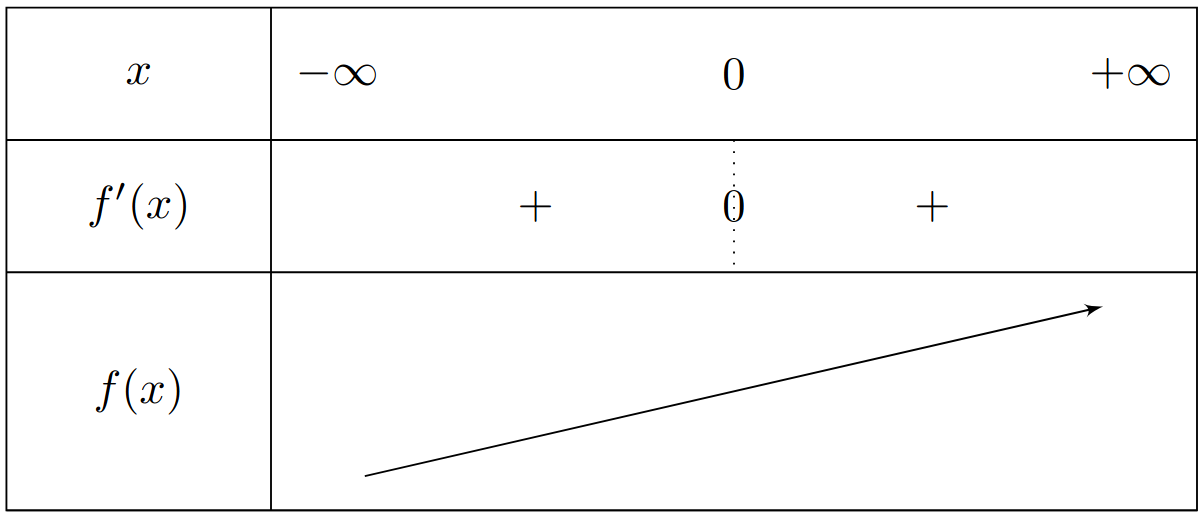
\includegraphics[width=0.5\textwidth]{swappy-20241228_160145.png}
\end{center}
\end{example}

\begin{example}
Étudier le sens de variation de $f: x \in \mathbb{R} \longmapsto-x^{3}+3 x+5$.
~\\Solution :\\
$f$ est dérivable sur $\mathbb{R}$ et pour tout $x \in \mathbb{R}, f^{\prime}(x)=-3 x^{2}+3$.\\
On étudie le signe de $f^{\prime}$ afin d'en déduire les variations de $f$ :\\
Pour cela, on commence par résoudre l'équation $f^{\prime}(x)=0$.\\
$x_{1}=1$ est une racine évidente de $-3 x^{2}+3=0$.\\
Le produit des racines est $\dfrac{c}{a}=\dfrac{-3}{3}=-1$ donc la seconde racine est $x_{2}=-1$.

Par ailleurs, comme $a=-3<0$, on en déduit le signe de $f^{\prime}$ :

\vspace{1em}
\begin{minipage}{0.65\linewidth}
\begin{center}
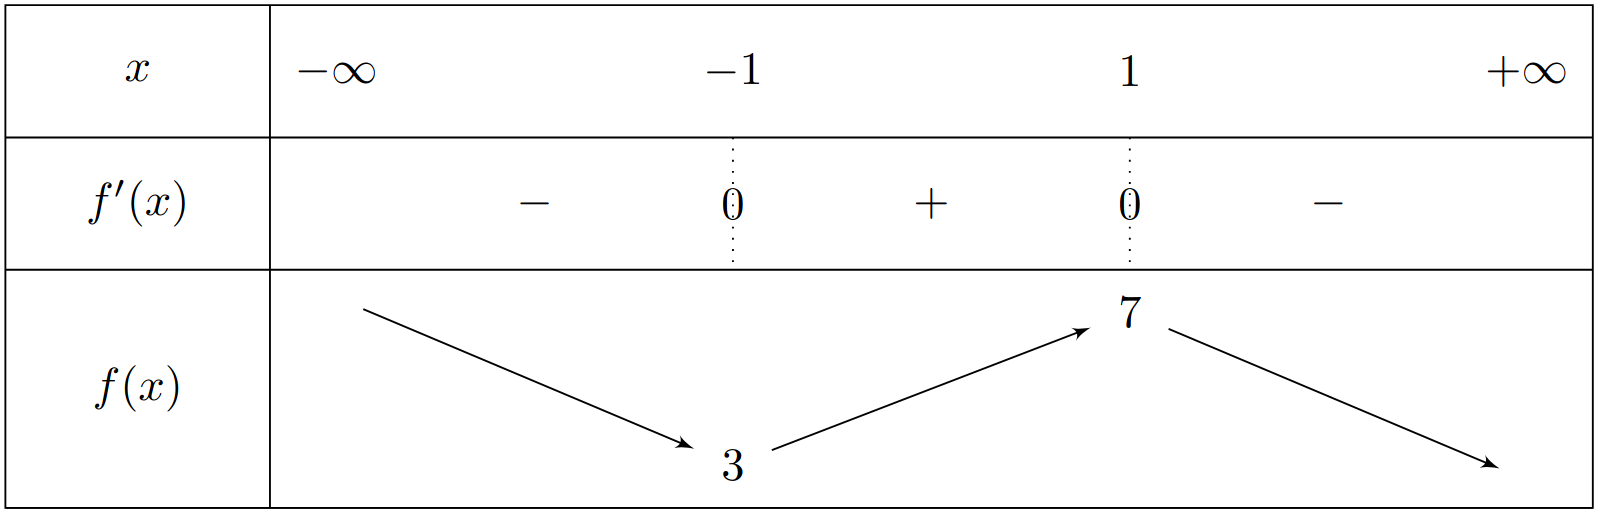
\includegraphics[width=1\linewidth]{swappy-20241228_160222.png}
\end{center}
\end{minipage}
\begin{minipage}{0.35\linewidth}
$$
\begin{aligned}
f(-1) & =-(-1)^{3}+3 \times(-1)+5 \\
& =3 \\
& \\
f(1) & =-1^{3}+3 \times 1+5 \\
& =7
\end{aligned}
$$
\end{minipage}
\end{example}

\section{Étude des extrema}
\begin{definition}{(Rappel)}{}
Soit I un intervalle et $c$ un réel de I . On considère une fonction $f$ définie sur I.\\
On dit que $f(c)$ est un \textbf{maximum global} sur I lorsque pour tout $x \in I, f(x) \leqslant f(c)$.\\
On dit que $f(c)$ est un \textbf{minimum global} sur I lorsque pour tout $x \in I, f(x) \geqslant f(c)$.
\end{definition}

\begin{definition}{}{}
Soit I un intervalle et $c$ un réel de I . On considère une fonction $f$ définie sur I .

\begin{itemize}
  \item Dire que $f(c)$ est un \textbf{maximum local} (respectivement \textbf{minimum local}) de $f$ signifie qu'il existe un intervalle $] a ; b[$ contenant $c($ avec $a \neq b)$ et tel que pour tout $x \in] a ; b[, f(x) \leqslant f(c)$ (respectivement $f(x) \geqslant f(c)$ ).
  \item Un \textbf{extremum local} est un maximum local ou un minimum local.\\
\end{itemize}
\end{definition}

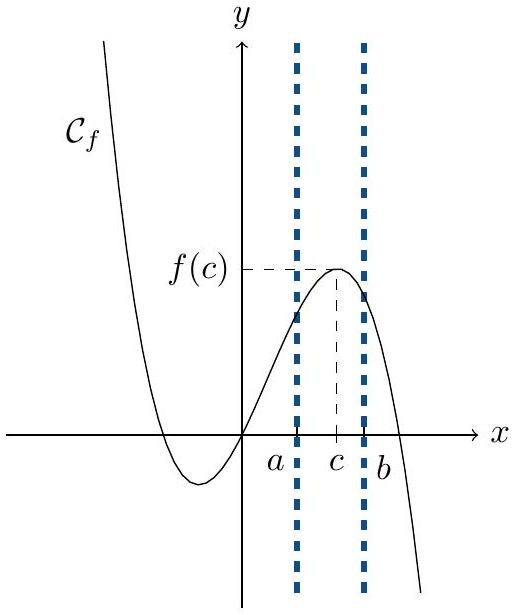
\includegraphics[max width=0.4\textwidth, center]{2024_12_28_241e70e4a27c0a7dff33g-3}

\newpage

\begin{proposition}{(admise)}{}
Soit $f$ une fonction définie sur un intervalle I et $c$ un réel de I .

\begin{itemize}
  \item Si $f(c)$ est un maximum global, alors $f(c)$ est un maximum local.
  \item Si $f(c)$ est un minimum global, alors $f(c)$ est un minimum local.
\end{itemize}
\end{proposition}

\begin{remark}
Les réciproques sont fausses!\\
Pour s'en convaincre, il suffit de considérer la fonction dont la courbe est représentée ci dessous. $f(1)=3$ est ici un maximum local mais n'est pas un maximum global.\\
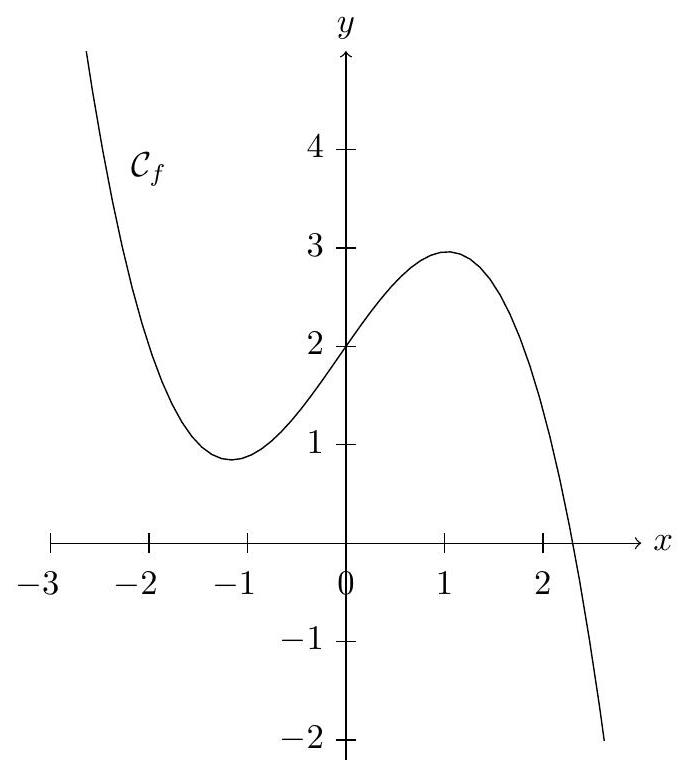
\includegraphics[max width=0.4\textwidth, center]{2024_12_28_241e70e4a27c0a7dff33g-4}
\end{remark}

\newpage

\begin{proposition}{(admise)}{}
Soit $f$ une fonction dérivable sur un intervalle ouvert I et $c$ un réel de I.

\begin{itemize}
  \item Si $f(c)$ est un extremum local, alors $f^{\prime}(c)=0$.
  \item Si $f^{\prime}$ s'annule en changeant de signes alors $f(c)$ est un extremum local de $f$.
\end{itemize}
\end{proposition}

\begin{remark}
\begin{itemize}
  \item[]
  \item L'hypothèse que l'intervalle I soit ouvert est indispensable.

Pour s'en convaincre, il suffit de considérer la fonction $f$ définie sur $[-1 ; 1]$ et dont la courbe est représentée ci-dessous. Cette fonction admet un maximum atteint en $x=1$ mais $f^{\prime}(1) \neq 0$.\\
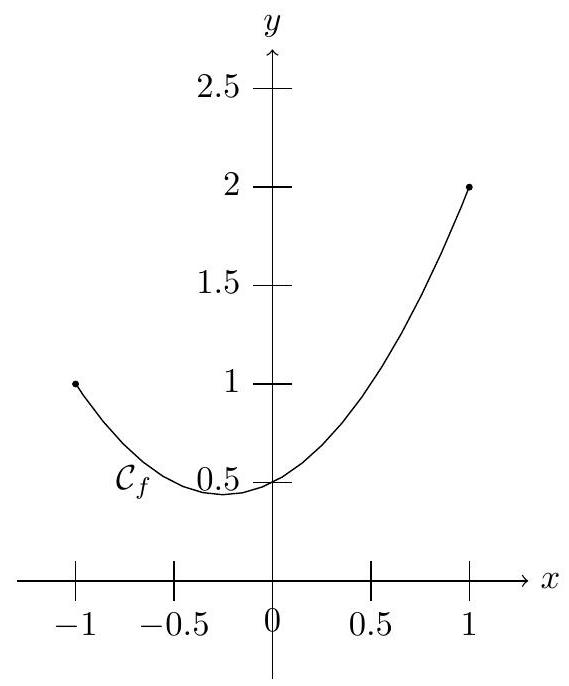
\includegraphics[max width=0.4\textwidth, center]{2024_12_28_241e70e4a27c0a7dff33g-5}

  \item L'hypothèse $f^{\prime}(c)=0$ n'est pas suffisante pour avoir un extremum local.

Par exemple, si $f: x \in \mathbb{R} \longmapsto x^{3}$, on a $f^{\prime}(0)=0$ mais $f$ n'admet pas d'extremum local en 0.
\end{itemize}
\end{remark}

\begin{savoir}{}{}
\begin{itemize}
  \item Étudier les variations d'une fonction.
  \item Déterminer des extremums locaux et globaux.
  \item Résoudre un problème d'optimisation.
  \item Exploiter les variations d'une fonction pour établir des inégalités.
\end{itemize}
\end{savoir}

\end{document}